\chapter{Edge focusing} \label{appendixedgefocusing} % For referencing this appendix elsewhere, use \ref{AppendixA}
\begin{figure}[htbp!]
	\centering
	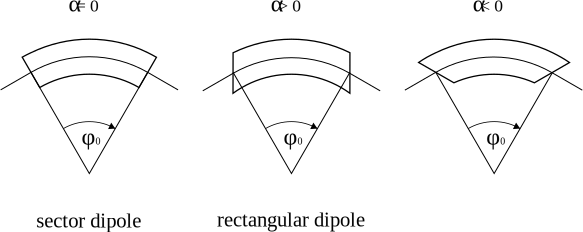
\includegraphics[width = \textwidth]{images/A-egde-focusing.pdf}
	\caption[Dipole magnets with different entrance and exit angles]{Dipole magnets with different entrance and exit angles (based on \cite{edge})}
	\label{fig:edge-angle-1}
\end{figure}
\noindent As shown in \autoref{fig:edge-angle-1} it possible to build dipole magnets with different entrance and exit angles~$\alpha$. Because of construction costs often rectangular magnets are used. The edge angle~$\alpha$ is defined in such a way that it is positive for a rectangular magnet. It influences the horizontal plane as well as the vertical plane and can be expressed due to a transfer matrix.

The effect on the horizontal motion is caused by changed path length within the dipole. As shown in \autoref{fig:edge-angle-2}, for a particle with a positive horizontal offset the path length is decreased by
\begin{figure}
	\centering
	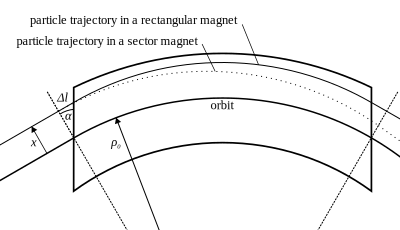
\includegraphics[width = 0.75\textwidth]{images/A-egde-focusing-horizontal.pdf}
	\caption{Edge focusing in the horizontal plane}
	\label{fig:edge-angle-2}
\end{figure}
\begin{align}
\Delta l = x \tan{\alpha} , 
\end{align}
while it is increased for a particle with negative horizontal offset. Therefore also the deflection angle $\varphi$ is changed:
\begin{align}
\Delta \varphi_{\textup{x}} = \frac{\Delta l}{\rho_{\textup{x0}}} = \frac{x \tan{\alpha}}{\rho_{\textup{x0}}} \quad \text{with} \quad \varphi_{\textup{x}} = \varphi_{0} - \Delta \varphi_{\textup{x}} 
\end{align}
As for small angles it is valid that
\begin{align}
\varphi_{\textup{x}} = \arctan{x'} \approx x', 
\end{align}
this can in thin lens approximation be written as a matrix:
\begin{equation}\begin{aligned}[b]
\textbf{R}_{\textup{edge,H}} = 
\begin{pmatrix} 
1 & 0 \\
\kap \tan{\alpha} & 1 \\
\end{pmatrix}
\end{aligned}\label{matrix-horizontaledgefocusing}\end{equation}
From \eqref{matrix-horizontaledgefocusing} we can see that the positive edge angle of a rectangular magnet leads to a defocussing in the horizontal plane. 

The vertical plane has a very similar matrix, even if it caused by a very different effect. The fringe fields of a dipole with an edge angle are not parallel to the orbit trajectory and have therefore also a horizontal component. This leads to the deflection angle 
\begin{figure}
	\centering
	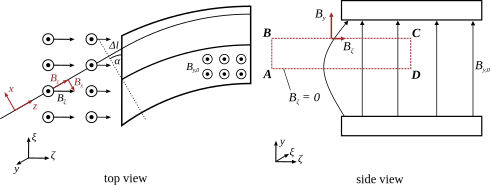
\includegraphics[width = \textwidth]{images/A-egde-focusing-vertical.pdf}
	\caption[Edge focusing in the vertical plane]{Edge focusing in the vertical plane (based on \cite{jankowiak})}
	\label{fig:edge-angle-3}
\end{figure}
\begin{align}
y' \approx \varphi_{\textup{y}} = \frac{q}{p} \int_{- \infty}^{+ \infty} B_{\textup{x}}(z) \du z 
\label{verticaldeflectionangle}\end{align}
in the vertical plane. As shown the in \autoref{fig:edge-angle-3} the horizontal field component can be written as
\begin{align}
B_{\textup{x}} = - \sin{\alpha} B_{\zeta}
\end{align}
We use the differential
\begin{align}
\du z = \frac{1}{\cos{\alpha}} \du \zeta
\end{align}
to substitute the integral of \eqref{verticaldeflectionangle}:
\begin{align}
\varphi_{\textup{y}} = - \frac{q \tan{\alpha}}{p} \int_{B}^{C} B_{\zeta}(\zeta) \du \zeta
\end{align}
As there are no magnetic monopoles we can use Gauss's law for magnetism
\begin{align}
0 = \oint \textbf{B} \du \textbf{r} = \int_{A}^{B} B_{\textup{y}} \du y + \int_{B}^{C} B_{\zeta} \du \zeta + \int_{C}^{D} B_{\textup{y}} \du y + \int_{D}^{A} B_{\zeta} \du \zeta,
\end{align}
where the first term is zero because of the field free region and the last term vanishes as $B_\zeta = 0$ in the symmetry plane. With
\begin{align}
\int_{B}^{C} B_{\zeta}(\zeta) \du \zeta = B_{\textup{y,0}} y
\end{align}
we obtain
\begin{align}
\varphi_{\textup{y}} = - \frac{q \tan{\alpha}}{p} B_{\textup{y,0}} y = - \kap \tan{\alpha}
\label{deflectionanglvertical2}\end{align}
for the vertical deflection angle. The matrix representation \eqref{deflectionanglvertical2} is given by:
\begin{equation}\begin{aligned}[b]
\textbf{R}_{\textup{edge,V}} = 
\begin{pmatrix} 
1 & 0 \\
-\kap \tan{\alpha} & 1 \\
\end{pmatrix}
\end{aligned}\label{matrix-verticaledgefocusing}\end{equation}

